\chapter{Physics at the ILC}

  In the chapter~\ref{chap:SM}, the framework of particles physics was described. 
  Since the beginning of High Energy Physics, different experiments have been done to confirm the exactness of the SM but also to find new physics beyond the SM. 
  The beam structure of the different colliders allow to perform different measurements with different precision. 
  For example, the LHC has a high luminosity and high energy beam, able to reach new energy scales on earth, whereas the ILC is trying to reach more precise results, with less energy. 
  Along this chapter, the physics scenarios that are going to be studied at the ILC are discussed. 
  Afterward, the emphasis will be on the Higgs physics and the measurement that would be performed at the ILC. 
  The last section aims to introduce a physics analysis scenario to study the processes which have a Higgs boson and two neutrinos in the final state.
 
 \minitoc

  \section{Potential studies}

  As seen in chapter \ref{chap:ILC}, the ILC will have a vast and variable tunable centre-of-mass energy.
  Due to the features of an $e^+e^-$ collider, the initial state of collision is well defined.
  Contrary to the LHC, there are no strong interaction backgrounds and the electroweak background is controlled and calculable.
  This conditions will help to perform precise measurements and looking for new physics. 
  The different measurements which will be performed are presented below.

   First of all, a study of the Z boson at the centre-of-mass energy of $\sqrt{s} = 91$ GeV around the Z resonance is scheduled. 
   This program called \textit{GigaZ} will be able to collect more Z boson events than the Large Electron Positron collider (LEP) did, because of a luminosity two to three times higher than what was achieved. 
   The data collected will allow a study on the asymmetries of the Z boson couplings. 
   A second program, called \textit{MegaZ}, will be performed at the centre-of-mass energy of $\sqrt{s} = 160$ GeV reaching the WW production threshold and trying to measure the W boson mass with a precision of $\text{MeV/c}^2$.
   At higher energy, it will also be possible to measure more precisely the W boson couplings.

   Afterward, the centre-of-mass energy will be adjusted to $\sqrt{s} = 250$ GeV to perform a study on the Higgs boson couplings, as well to measure its the quantum numbers.
   At this energy, the Higgs boson is mainly procduced via Higgs-strahlung.
   The measurement is done thanks to the recoil mass independently of the Higgs decay products.
 
   Then, for a centre-of-mass energy between 350 and 400 GeV, two studies are achievable. 
   The WW-fusion process starts to rise and permits to measure the couplings of the Higgs boson to the W ones in order to look for deviation from the Standard Model. 
   Moreover, this channel allows to study some rare decays. 
   This energy range corresponds also to the threshold of the top quark pairs production.
   Because of the top quark life-time, the two quarks created are not in a bounded-state. 
   By performing a threshold scan, the mass of the top quark can be measured with a precision reaching 100 $\text{MeV/c}^2$.

   The nominal energy of the \gls{ILC} is achieved at $\sqrt{s} = 500$ GeV.
   This energy scale is suitable to look for supersymmetry candidates and possible extended states of the Higgs boson.

   An upgrade of the ILC to reach the centre-of-mass energy $\sqrt{s} = 1$ TeV is also scheduled.
   Up to 1 TeV, new measurements are possible, such as the coupling of the Higgs boson to the top quark, the Higgs boson self-coupling, or is compositeness.
   Although, search for new exotic particles and physics beyond the \gls{SM} is possible.
    
   The table~\ref{tab:physicsAtIlc} summarises the different physics programs at the ILC for the different energy reachable.  

  \begin{table}[h]
    \begin{center}
    \begin{tabular}{c c c}
      \hline %----------------------------
      Energy (GeV) &  Reaction  &  Physics Goal \tabularnewline
      \hline %----------------------------
      \hline %----------------------------
      91  &  $e^+e^- \rightarrow Z $ & ultra-precision electroweak \tabularnewline
      \hline %----------------------------
      160 & $e^+e^- \rightarrow WW $ & ultra-precision W mass \tabularnewline
      \hline %----------------------------
      250 & $e^+e^- \rightarrow Zh$ & precision Higgs coupling \tabularnewline
      \hline %---------------------------- 
      \multirow{3}*{350 - 400} & $e^+e^- \rightarrow t\overline{t}$ & top quark mass and couplings \tabularnewline
                               & $e^+e^- \rightarrow WW $ & precision W couplings \tabularnewline
                               & $e^+e^- \rightarrow \nu\overline{\nu}h$ & precision Higgs couplings\tabularnewline
      \hline %----------------------------
      \multirow{5}*{500} & $e^+e^- \rightarrow f\overline{f}$ & precision search for Z' \tabularnewline
                         & $e^+e^- \rightarrow t\overline{t}h $ & Higgs coupling to top \tabularnewline
                         & $e^+e^- \rightarrow Zhh $ & Higgs self-coupling \tabularnewline
                         & $e^+e^- \rightarrow \tilde{\chi}\tilde{\chi} $ & search for supersymmetry  \tabularnewline
                         & $e^+e^- \rightarrow AH, H^+ H^-$ & search for extended Higgs states \tabularnewline
      \hline %----------------------------
      \multirow{4}*{700-1000} & $e^+e^- \rightarrow \nu\overline{\nu}hh$ & Higgs self-coupling\tabularnewline
                              & $e^+e^- \rightarrow \nu\overline{\nu}VV$ & composite Higgs sector\tabularnewline
                              & $e^+e^- \rightarrow \nu\overline{\nu}t\overline{t}$ & composite Higgs and top\tabularnewline
                              & $e^+e^- \rightarrow \overline{t}\overline{t}^*$ & search for supersymmetry\tabularnewline
      \hline %----------------------------
    \end{tabular}
    \end{center}
      \caption{Summary of the major processes that will be studied at the ILC for different energies\cite{Baer2013}.}
      \label{tab:physicsAtIlc}
  \end{table}
  
  \section{Higgs physics}

  The Higgs boson found at the \gls{LHC} has to be characterised more precisely.
  One of the goal study at the \gls{ILC} is to determine if the particle found is compatible with the one defined by the Standard Model, or if other states exist.
  The measurement of the Higgs boson couplings to the Standard Model particle is one of the key to verify the exactness of the mass generation mechanism described by this theory and to open the door to any proof of physics beyond the Standard Model.
  The production, the decay modes of the Higgs boson, as well as the measurement feasible are presented below in the case of the \gls{ILC}.


    \subsection{Production of the Higgs at the ILC}

    Due to the beam structure at the \gls{ILC}, the Higgs boson is accessible by direct measurement.
    The production of the Higgs boson defined by the Standard Model is done via three major processes: the Higgs-strahlung (see figure~\ref{fig:higgsStrahlung}), the WW-fusion (see figure~\ref{fig:WW-fusion}) and the ZZ-fusion (see figure~\ref{fig:ZZ-fusion}).

    \begin{description}
      \centering
      \item[Higgs-strahlung:] $e^+e^- \rightarrow ZH \rightarrow f\overline{f}X$
      \item[WW-fusion:] $e^+e^- \rightarrow \nu \overline{\nu} W^+W^- \rightarrow \nu \overline{\nu} H$
      \item[ZZ-fusion:] $e^+e^- \rightarrow e^+e^- ZZ \rightarrow e^+e^- H$
    \end{description}

    The figure~\ref{fig:higgsProduction} summarises the different Feynman diagrams of the Higgs boson production.

    At the centre-of-mass energy $\sqrt{s} = 250$ GeV, the Higgs-strahlung is the dominant process and occurs via a s-channel. 
    Its cross-section falls off as 1/s as the centre-of-mass energy $\sqrt{s}$ increases.
    Contrary to the Higgs-strahlung, the WW-fusion and the ZZ-fusion are t-channel processes which have a cross-section growing logarithmically with the centre-of-mass energy.
    Thus, at 250 GeV, the cross-section of the WW-fusion is one order smaller than the Higgs-strahlung and the ZZ-fusion is negligible.
    Nevertheless, around 500 GeV, the WW-fusion and the Higgs-strahlung have the same cross-section, which is around 120 fb.
    The figure~\ref{fig:higgsXsec} shows the cross-section production of the Higgs at the ILC regarding the energy of the collision.
    
    \begin{figure}  
        \centering
        \begin{subfigure}[t]{0.3\textwidth}
            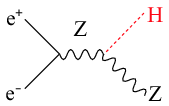
\includegraphics[width = 0.85\textwidth]{Pictures/Higgs/Chapter_Theory_figs_ZHdiagram.png}
            \caption{Higgs-Strahlung}
            \label{fig:higgsStrahlung}
        \end{subfigure}
        ~%\qquad
         %add desired spacing between images, e. g. ~, \quad, \qquad, \hfill etc. 
          %(or a blank line to force the subfigure onto a new line)
        \begin{subfigure}[t]{0.3\textwidth}
            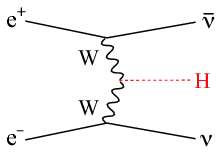
\includegraphics[width = 0.85\textwidth]{Pictures/Higgs/Chapter_Theory_figs_nunuHdiagram.png}
            \caption{WW-fusion}
            \label{fig:WW-fusion}
        \end{subfigure}
        ~%\qquad
         %add desired spacing between images, e. g. ~, \quad, \qquad, \hfill etc. 
          %(or a blank line to force the subfigure onto a new line)
        \begin{subfigure}[t]{0.3\textwidth}
            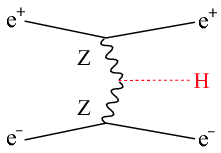
\includegraphics[width = 0.85\textwidth]{Pictures/Higgs/HiggsProd_eeH.png}
            \caption{ZZ-fusion}
            \label{fig:ZZ-fusion}
        \end{subfigure}
        \caption{Feynman diagrams of the main Higgs production at the ILC\cite{Asner2013}\cite{tian}.}
        \label{fig:higgsProduction}
    \end{figure}    
    
    The WW-fusion occurs only with left-handed electrons associated to right-handed positrons.
    Thus, by modifying the beam's polarisation, the signal mixture can be changed, as well as the background processes.

    \begin{figure}[!h]
      \centering
      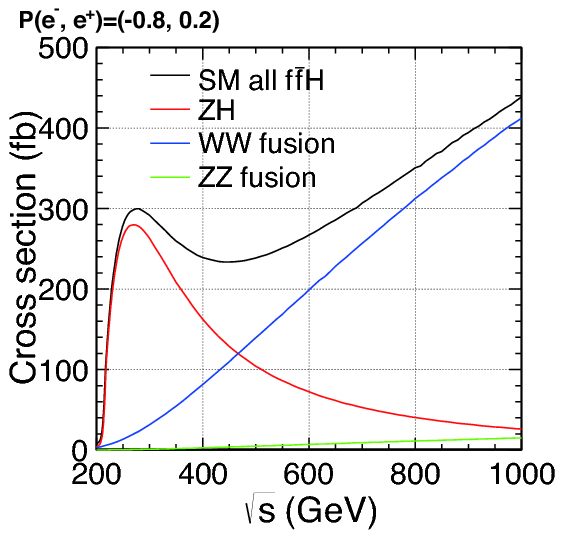
\includegraphics[width = 0.65\textwidth]{Pictures/Higgs/higgs_xsec_P-8_3.png}
      \caption{The cross section production of the Higgs boson with a mass of 125 GeV\cite{Asner2013}.}
      \label{fig:higgsXsec}
    \end{figure}

       
    \begin{figure}[!h]
      \centering
      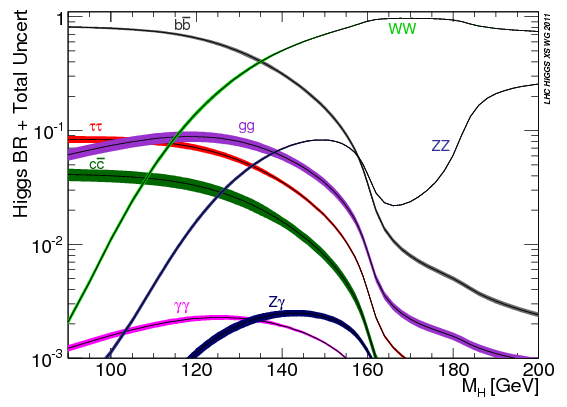
\includegraphics[width = 0.7\textwidth]{Pictures/Higgs/BRTotalUncertBands_lm.png}
      \caption{The Higgs branching ratio with the branching ratio uncertainties for the Higgs mass varying from 80 to 200 GeV\cite{Denner:2011mq}.}
      \label{fig:higgsProd}
    \end{figure}

    \subsection{Decays of the Higgs}

    At the \gls{LHC}, only the decay $H \rightarrow b\overline{b}$ is observed under special kinematics. 
    The other decay states are challenging to separate from the background.
    Thanks to the properties of the \gls{ILC} beams, the couplings of the Higgs to the particles of the \gls{SM} is measurable.
    Thus, the following decay are available: $b\overline{b}$, $WW$, $ZZ$, $gg$, $c\overline{c}$, $\tau \tau$, $\gamma \gamma$, $\gamma Z$.
    The observation of the $H \rightarrow c\overline{c}$ is one of the constraint parameter to build the detectors, specifically, the vertex detector that should be able to distinguish the vertices coming from the $b$-quarks to the ones coming from the $c$-quarks.
    The figure~\ref{fig:coupling} depicts the mass-coupling relation of the Higgs boson to the particles of the \gls{SM}.
    The \gls{SM} nature of the Higgs boson will be tested by looking for any deviations from its fermionic coupling.
    A deviation might indicate multiple states for the Higgs boson. \todo{Not clear enough}

    \begin{figure}[!h]
      \centering
      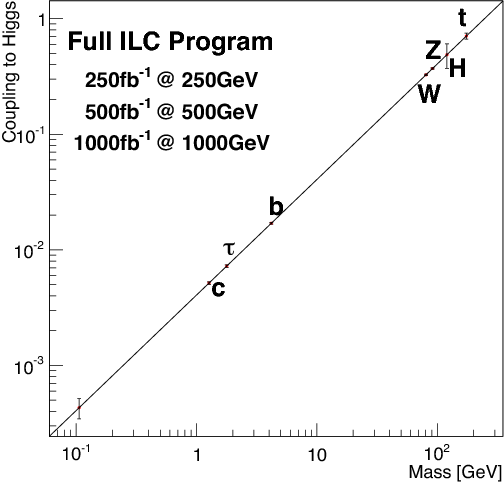
\includegraphics[width = 0.5\textwidth]{Pictures/Higgs/Chapter_Theory_figs_mass-coupling1TeV.png}
      \caption{Mass-coupling relation of the Higgs boson to the particles defined in the standard model\cite{tian}.}
      \label{fig:coupling}
    \end{figure}

    \subsection{Higgs studies}

    The first study will be at the peak production of the Higgs-strahlung. 
    The well defined four-momentum initial state allows to measure the Higgs boson mass regardless its decay products.
    The Higgs invariant mass $M_H$ can be calculated by using the recoil technique:

    \begin{equation}
      M^2_H = s + M^2_Z - 2 \sqrt{s}\left(E_{1} + E_{2}\right)
    \end{equation}

    Where $M_Z$ is the mass of the Z boson, $E_1$ and $E_2$ are the energy of the Z decay products. 
    This technique works well for the Z boson decaying into leptons at the centre-of-mass energy $\sqrt{s} = 250$ GeV.
    However, at this centre-of-mass energy, this method can not be performed for a Higgs decaying into quarks. 
    The Z boson and the Higgs boson are produced almost at rest, thus, the identification of the jets coming from the Z boson to the ones coming from the Higgs boson is more difficult.
    Nevertheless, at higher energy ($\sqrt{s} = 500$ GeV), the two bosons are enough boosted to separate their jets and ten to apply again the recoil mass.
    Depending on the decay channel of the Z bosons, the statistical precision on the mass measurement varies between 40 MeV (for $Z \rightarrow \mu^+\mu^-$) to 80 MeV (for $Z \rightarrow e^+e^-$) and can reach 32 MeV by combining the two results.

    The spin and CP measurement are also going to be performed. 
    The LHC has excluded the possibility of spin 1 boson, thanks to the measurement of the di-photon channel. 
    At a centre-of-mass energy $\sqrt{s} = 250$ GeV, the cross-section of the higgs-strahlung depends on the spin and CP numbers.
    For example, if the spin is 0 and the CP even, the cross-section s
    If spin 0 and CP-odd: cross section
    


  \section{Analysis of simulated data}
  
    Due to the restricted time to conduct the thesis, this section is introducing the tools to perform an analysis of some simulated data at the ILD. 
    The results shown are not the latest and were already demonstrated. 
    Nevertheless, the philosophy to perform a study of the Higgs production at the center-of-mass energy $\sqrt{s} = 350$ GeV and a luminosity of 250 $\text{fb}^{-1}$ is here presented.
  
  \section{Simulation set-up}  
  
    Monte Carlo simulation and analysis software framework were developed for the linear collider community.

    \subsubsection{ILCSoft}
    
    The ILCSoft provides a large variety of software packages which were developed for the linear collider community\cite{ilcsoft}.
    It includes software for Monte-Carlo simulation, as software for test beam analysis (see section ??) and other tools.
    The main package is the \gls{LCIO}, a persistency framework and event data model for the linear collider detector studies\cite{lcio}. 
    It provides a common data format and event data model for both the simulation studies and the analysis framework in order to share results and compare reconstruction algorithms.
    A C++ software framework called \gls{Marlin} is used for the reconstruction and the analysis by using the \gls{LCIO} data format.
    Each tasks are structured into module called processors. 
    A steering file written in XML is used to select the processors to use and the order of their execution time.
    An other package is \gls{GEAR}.
    It is use as a geometry detector toolkit.
    A steering file is in charge to perform the interface of the detector geometry during the data reconstruction and the analysis.

    The Monte-Carlo simulation is performed in three steps.
    The first one consists to generate the physics events of electron/positron collisions.
    The generation of Mont-Carlo events are performed with WHIZARD.
    This software includes Standard Model processes, as well as a large variety of BSM models.
    For the purpose of the \gls{ILC}, it can simulate the beamstrahlung, the \gls{ISR} and the beam polarisation.
    Although the hard interaction are simulated thanks to WHIZARD, the hadronisation and fragmentation are implemented via PYHIA.
    
    Afterward the physics events are generated, the particle interaction inside the detector is simulated with MOKKA.
    The software is based on GEANT4 simulation toolkit and is par of the ILCSoft.
    For the analysis, the detector model used is ILD\_o1\_v05.
    This model simulates the dead areas due to cabling, cooling system and mechanical structure and has a silicon-tungsten electromagnetic calorimeter, as well as an analog hadronic calorimeter.
    
    Finally, the events are reconstructed thanks to Marlin.

  \subsection{Background processes}

    The hypothesis is to have a final state consisting of two jets coming from the decay of the Higgs boson plus missing energy from two neutrinos.
    Are considered as background, the events with the same final states as the signal and the events with a similar detector response.

   
   \begin{description}
      \item[W-boson pair production] 
      \begin{itemize}
        \item Semi-leptonic decay
        \item Hadronic decay
      \end{itemize}
      \item[Z-boson pair production]
      \begin{itemize}
        \item Hadronic decay
        \item Leptonic decay
        \item Hadronic decay with missing energy
      \end{itemize}
      \item[Single W-boson production]
      \item[Single Z-boson production]
      \begin{itemize}
        \item Hadronic decay
        \item Hadronic and electron/positron decay
      \end{itemize}
      \item[Higgs-strahlung]
      \begin{itemize}
        \item Hadronic decay
        \item Leptonic decay
      \end{itemize}
   \end{description}
 
  \subsection{Event reconstruction}

  \begin{itemize}
    \item Identification of isolated leptons to remove some of the background processes
    \item Look for jet-like objects in the forward region corresponding to low pT hadrons coming from $\gamma \gamma$ interactions.
    \item Jet clustering and flavor tagging
  \end{itemize}

  \subsection{Event selection}
